\chapter{Partitioned Element Methods} \label{ch:pem}
%
This chapter defines a general class of polytopal element formulations referred to as partitioned element methods (PEM). The essential characteristics and mathematical requirements placed upon these methods are formally stated, giving rise to a family of different approaches, for which some formal investigations are conducted in subsequent chapters. Several specific formulations are summarized in detail, and a number of existing methods are herein classified as particular instances of partitioned element methods.

\section{Overview}

	% reiterate the desire for robust, arbitrary polytopal elements
	% reiterate the shortcomings of generalized barycentric coordinates
	% reiterate the shortcomings of VEM
	% PEM considers the construction of shape functions to be a special type of local approximation problem
		% need to determine well-behaved interpolants on element domains
		% can pose this as a boundary value problem
		% approximate its solution using existing methods (FEM, etc.)
		% yields relatively simple representation of shape functions
			% i.e. piece-wise polynomial
		% may utilize the discretization to define simple quadrature rules
			% e.g. composite mid-point rules
			% can enhance accuracy of these rules using gradient correction
	% Some questions:
		% how refined must the element's local discretization be to matain a sufficient level of accuracy?
			% is a coarse discretiztion sufficient?
		% what BVP should be used?
			% Laplace's equation? (harmonic SFs)
			% specification of BVP determines quality/robustness of SFs
		% are certain approximation methods more suitable than others?
			% FEM? DG? VEM?

Partitioned element methods are finite element-like methods which approach the task of constructing shape functions on arbitrary polytopal element domains by partitioning each element into sub-domains (quadrature cells). The element partition serves a dual purpose: it is used to establish a composite quadrature rule for the element, and to define a finite dimensional function space, from which the element's shape functions are selected as the solutions to corresponding boundary value problems, defined locally on the element.

	% want efficient and stable quadrature rules
Partitioned element methods are motivated by the idea that it is generally easier and more efficient to define complicated functions over arbitrary domains if the functions are defined in a piecewise polynomial fashion over simpler sub-domains. This is precisely the mentality which likewise motivates the finite element method and other related numerical approximation methods.

The PEM is driven by the need for establishing stable and efficient quadrature rules on arbitrary polytopes. Unlike virtual element methods which typically circumvent the use of quadrature altogether, partitioned element methods recognize the necessity of using domain quadrature rules to evaluate nonlinear residual and stiffness contributions. The use of sufficient quadrature also yields a stable integration of the weak form which does not rely upon unphysical stabilization parameters.

	% depart from the idea of shape functions defined pointwise
In contrast with traditional perspectives which regard the shape functions as being continuously defined on element domains (i.e. generalized barycentric coordinates), the PEM exploits the fact that the shape functions and their gradients only need to be evaluated at a discrete number of quadrature points. With this in mind, PEM approximation spaces are deliberately constructed around the quadrature cell partition of the element, and consequently resemble finite element approximation spaces.

	% enforce constraints to attain reproducibility & consistency
The resulting shape functions on each element are altogether subject to the conditions of approximability, compatibility, stability, and quadrature consistency, as discussed in chapter \ref{ch:solid_mechanics}. Together, these conditions impose a number of unique requirements upon the element's partition, it's corresponding quadrature rules, and the associated cell-based approximation spaces.

In the following sections, an abstract framework for the PEM is established, describing the shape function boundary value problems defined on an element, and their corresponding approximations. We further enumerate several specific partitioned element methods, and provide an assessment of their potential strengths and weaknesses.

%PEM encompasses the special case where each element consists of a single sub-domain. Such approaches will henceforth be referred to as \textit{single-cell} methods, which share certain similarities with the VEM and VETFEM. Single-cell methods are not particularly robust when applied to arbitrary polyhedral meshes (namely those generated by B-rep intersection); they perform poorly if the element's geometry is sufficiently complicated.

\section{Definition of Element Shape Functions}

	Consider the structure of a polyhedral element $\Omega \subset \mathbb{R}^3$, as depicted in Figure \ref{fig:polyhedral_element}. The element's boundary $\partial \Omega$ may be subdivided into a set of polygonal faces $\mathcal{T}_F (\Omega) = \left\{ F_i \right\}_{i=1}^{N_F}$, such that each face $F_i$ is shared entirely with an adjacent element, or with the mesh boundary. Corresponding sets of linear edges $\mathcal{T}_E (\Omega) = \left\{ E_i \right\}_{i=1}^{N_E}$ and nodes $\mathcal{T}_V (\Omega) = \left\{ V_i \right\}_{i=1}^{N_V}$ result by considering the sets of all unique intersections $\mathcal{T}_E (\Omega) = \left\{ \partial F_i \cap \partial F_j \neq \emptyset \, \, \forall i \neq j \right\}$ and $\mathcal{T}_V (\Omega) = \left\{ \partial E_i \cap \partial E_j \neq \emptyset \, \, \forall i \neq j \right\}$, respectively.
	
\begin{figure} [!ht]
	\centering
	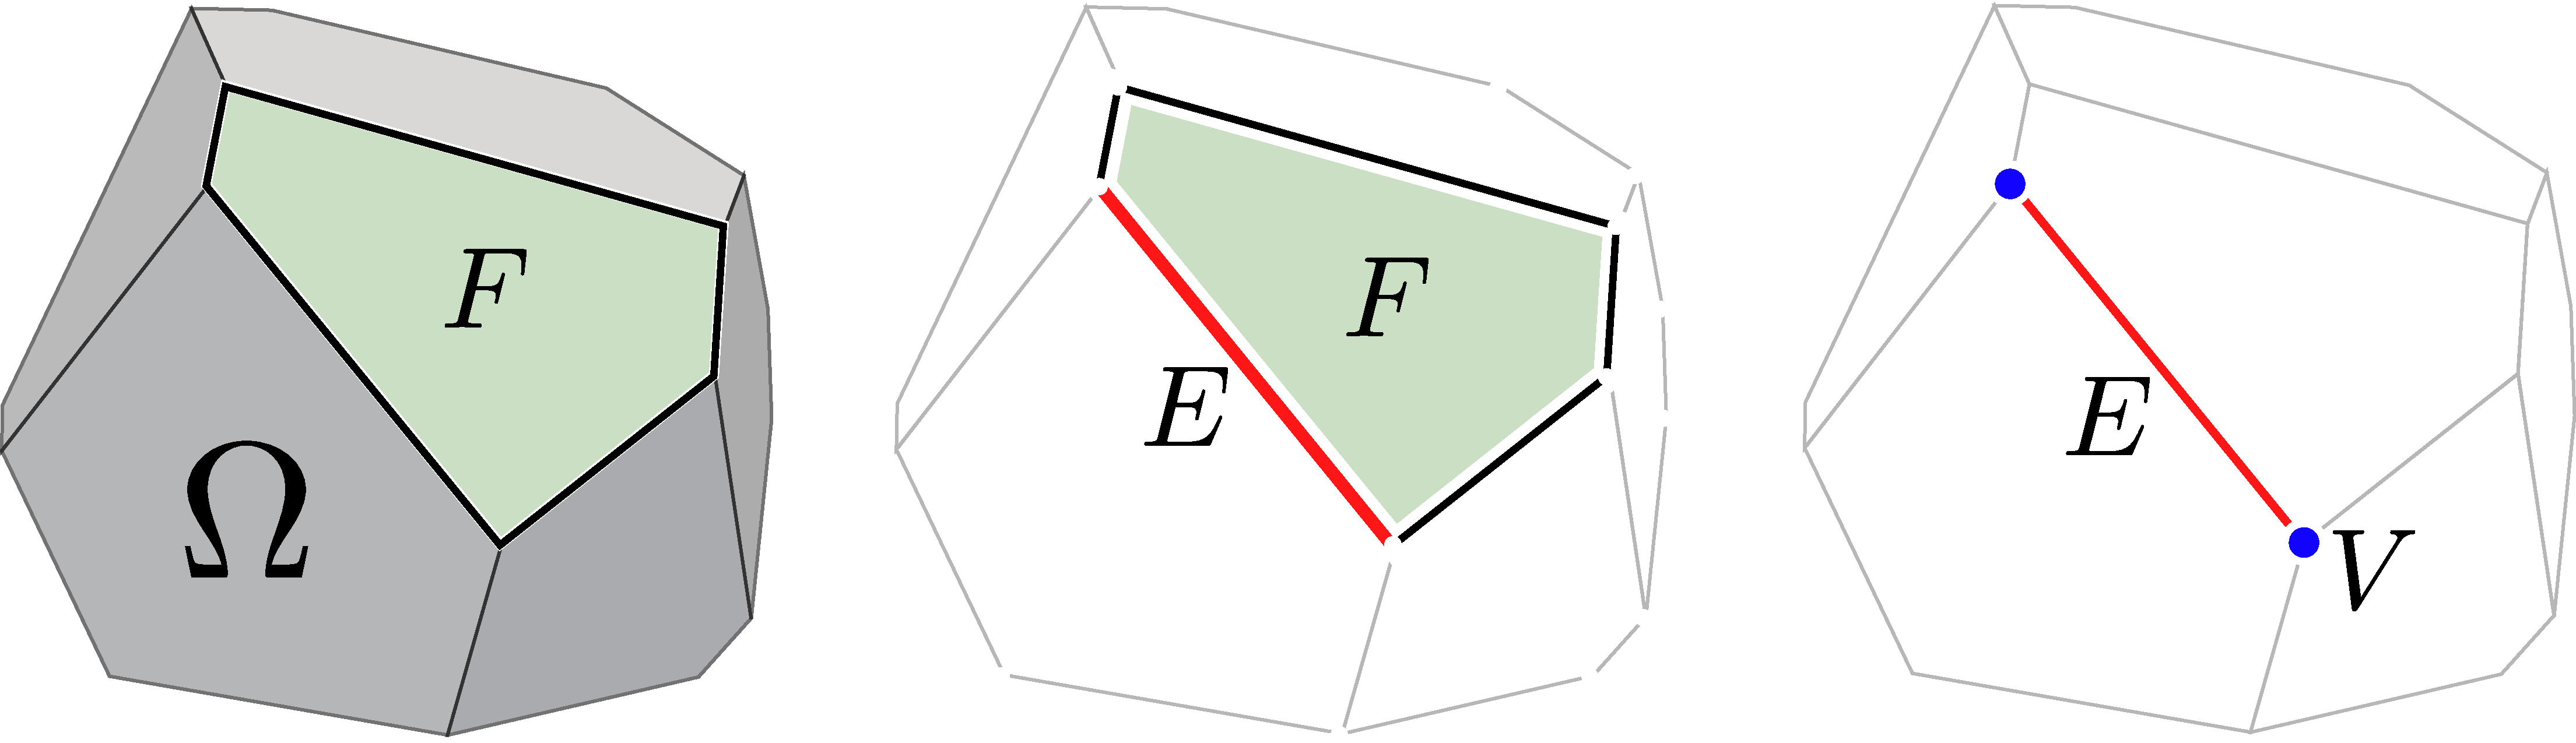
\includegraphics[width = 6.0in]{figures/polyhedron_decomposition.pdf}
	\caption{A representative polyhedral element $\Omega \subset \mathbb{R}^3$, and it's corresponding sets of faces, edges, and nodes.}
	\label{fig:polyhedral_element}
\end{figure}
	
	% PEM function spaces are broken $H^1 (\Omega)$ spaces
	% functions are defined independently on the open interior $\Omega$
	% functions defined independently on shared element interfaces
	The function spaces to which the element's shape functions belong are effectively broken Sobolev spaces, where a given shape function $\varphi \in \mathcal{W}_k (\overline{\Omega})$ is defined independently on the open interior of each polyhedral element $\Omega \subset \mathbb{R}^3$, and on its boundary $\partial \Omega$, such that
	\begin{equation}
		\mathcal{W}_k (\overline{\Omega}) = \left\{ \varphi|_{\Omega} \in H^k (\Omega) : \mathcal{L}_{\Omega} \varphi = f_{\Omega} \, \text{in} \, \Omega, \, \varphi|_{F} \in \mathcal{W}_k (\overline{F}) \, \, \forall F \in \partial \Omega \right\},
	\end{equation}
	\begin{equation}
		\mathcal{W}_k (\overline{F}) = \left\{ \varphi|_{F} \in H^k (F) : \mathcal{L}_{F} \varphi = f_{F} \, \text{in} \, F, \, \varphi|_{E} \in \mathcal{W}_k (\overline{E}) \, \, \forall E \in \partial F \right\},
	\end{equation}
	\begin{equation}
		\mathcal{W}_k (\overline{E}) = \left\{ \varphi|_{E} \in H^k (E) : \mathcal{L}_{E} \varphi = f_{E} \, \text{in} \, E, \, \varphi|_{V} \in \mathbb{R} \, \, \forall V \in \partial E \right\}.
	\end{equation}
	In essence, a given function $\varphi|_{\Omega} \in H^k (\Omega)$ defined on the element's interior is related to a corresponding boundary function $\varphi|_{\partial \Omega} = \bar{\varphi}$ (which itself is a broken $H^k (\partial \Omega)$ function) via a well-posed Dirichlet boundary value problem:
	\begin{equation}
		\mathcal{L}_{\Omega} \varphi = f_{\Omega} \quad \forall \mathbf{X} \in \Omega \quad \text{s.t.} \quad \varphi = \bar{\varphi} \quad \forall \mathbf{X} \in \partial \Omega,
		\label{eq:pem_bvp}
	\end{equation}
	where $\mathcal{L}_{\Omega}$ denotes a linear differential operator, and $f_{\Omega} \in L^2 (\Omega)$ is a generic forcing function. The element's degrees of freedom are collectively accounted for in the boundary function $\bar{\varphi}$ and the forcing function $f_{\Omega}$. Consequently, the interior function $\varphi|_{\Omega}$ is uniquely defined, provided there exists a unique solution to (\ref{eq:pem_bvp}). In turn, we suppose that $\varphi|_{F} \in H^k(F)$ is the solution to a similar (2-dimensional) boundary value problem defined on each face $F$, and $\varphi|_E \in H^k(E)$ is the solution to a (1-dimensional) BVP on each edge $E$.
	
	% Additionally, the PEM considers the boundary of each element to be partitioned into a collection of $2$-dimensional polygonal faces $\partial \Omega = \cup_{i = 1}^{N_F} F_i$, where a given face $F$ is either a shared interface between two elements $F = \partial \Omega_a \cap \partial \Omega_b \neq \emptyset$ ($a \neq b$), or else it is a part of the domain boundary $F \subset \partial \Omega_a \cap \partial \mathcal{B}_0 \neq \emptyset$.
	% The boundary of each face $\partial F$ is likewise recursively partitioned into $1$-dimensional edges $\partial F = \cup_{i = 1}^{N_E} E_i$, whose end-points are the geometric verticies (the nodes) of the polyhedral element in question, which bear the primary degrees of freedom.
	
	The advantage of defining shape functions in this manner is that it affords a great deal of flexibility in the construction of arbitrary order interpolants (or enhancement functions), while maintaining $C^0 (\mathcal{B}_0)$ continuity at inter-element interfaces. Moreover, given that the shape functions are uniquely defined at every point $\mathbf{X} \in \Omega$, they are amenable to post-processing and visualization-related tasks.
	
%	In the following sections, we will explore a few specific choices for the differential operator $\mathcal{L}$ and the forcing functions $f$ defined on the element and its faces, etc.

\subsection*{Harmonic Shape Functions}

	% Ideally want the shape functions to be uniquely defined on polytopes
	% This can be achieved by considering SFs as unique solutions to BVPs
	% Most natural BVP to consider is Laplace's equation with Dirichlet BCs
	% BCs arise from conditions of compatibility with nodal values
		% Help to guarantee weak inter-element compatibility
	% Other authors have explored the idea of harmonic SFs on polytopes
		% See \cite{Gordon:74}, \cite{Martin:08}, \cite{Bishop:14}
		% To obtain these SFs, the authors use an element partition
	% In previous works, the BCs were enforced as closely as possible
	% This is not necessarily a good thing
		% The solution to Laplace's equation can yield sharp gradients
		% On arbitrary domains, can result in poor conditioning, locking
	% In the present work, we seek to relax the conditions of compatibility
		% Consider weak compatibility requirements
			% Develop notion of weak compatibility in a rigorous setting
			% Establish weak compatibility as sufficient for convergence
			% Examine necessary conditions for stability
		% Yields a non-conforming finite element method
		% Elements are more robust on account of relaxed compatibility
		% Polytopes accomodate nonconformity better (than simplicies, etc)

	The simplest choice of $\mathcal{L}_{\Omega} = -\nabla^2$ and $f_{\Omega} = 0$ corresponds to Laplace's equation:
	\begin{equation}
		\nabla^2 \varphi = 0 \quad \forall \mathbf{X} \in \Omega \quad \text{s.t.} \quad \varphi = \bar{\varphi} \quad \forall \mathbf{X} \in \partial \Omega,
		\label{eq:pem_laplace}
	\end{equation}
	whose solution $\varphi$ is harmonic on $\Omega$ (and likewise on each face $F$ and edge $E$ -- refer to Figure \ref{fig:harmonic_sfs}). Harmonic shape functions form a partition of unity, are linearly complete, and arise from degrees of freedom $\varphi|_V$ borne only by the nodes of each element; therefore, they satisfy the kronecker delta property. As such, harmonic shape functions are classifiable under the category of generalized barycentric coordinates.
	
\begin{figure} [!ht]
	\centering
	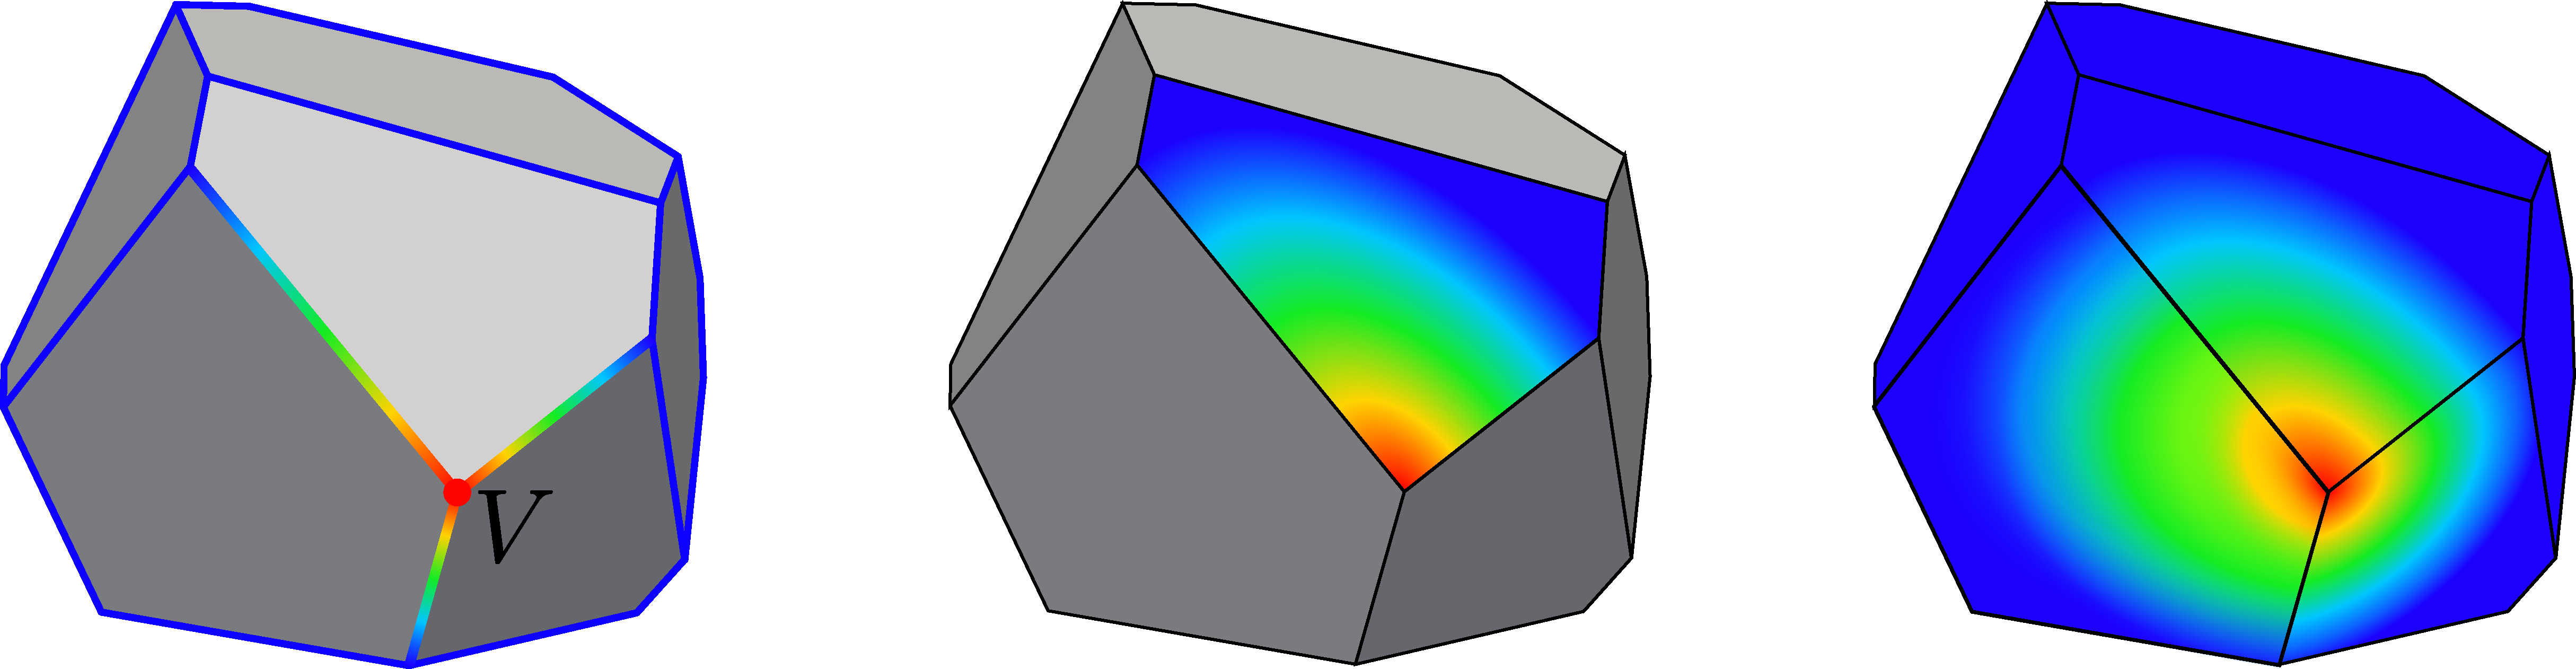
\includegraphics[width = 6.0in]{figures/harmonic_sfs.pdf}
	\caption{The harmonic shape function corresponding to a given node, defined hierarchially on each edge, face, and the element.}
	\label{fig:harmonic_sfs}
\end{figure}
	
	If instead $f_{\Omega} \neq 0$ (corresponding to Poisson's equation), then
	\begin{equation}
		-\nabla^2 \varphi = f_{\Omega} \quad \forall \mathbf{X} \in \Omega \quad \text{s.t.} \quad \varphi = \bar{\varphi} \quad \forall \mathbf{X} \in \partial \Omega,
		\label{eq:pem_poisson}
	\end{equation}
	and we may introduce additional degrees of freedom through $f_{\Omega}$ belonging to edges, faces, or element domains. These degrees of freedom are not necessarily associated with nodal evaluations of $\varphi$, but instead may be designed to exhibit certain desirable characteristics (to recover a particular order of polynomial completeness). The solution $\varphi$ to (\ref{eq:pem_poisson}) is not harmonic; instead, we shall refer to functions which satisfy (\ref{eq:pem_poisson}) as \textit{generalized harmonic shape functions}.
	
	Harmonic shape functions are not a new concept; Gordon and Wixom were among the first authors to propose the idea in \cite{Gordon:74}, and Martin et al. later considered their application to polyhedral finite elements in \cite{Martin:08}. However, obtaining exact solutions to (\ref{eq:pem_laplace}) is generally infeasible for arbitrary polyhedra. In practice, approximate solutions must be considered.
	
	In particular, Bishop has proposed a method for constructing FE approximations to harmonic shape functions in \cite{Bishop:14}. Additionally, the VETFEM (\cite{Rashid:00}, \cite{Rashid:06}) and the original PEM presented in \cite{Rashid:12}, may be viewed as techniques for obtaining discrete approximations to harmonic shape functions. Likewise, many virtual element methods (\cite{Chi:17}, \cite{Veiga:13}, \cite{Veiga:15}) suppose that the element shape functions are harmonic over individual element domains, though they are never explicitly constructed or represented as such.
	
	It herein becomes of interest to determine suitable approximations to harmonic shape functions on arbitrary polyhedra. A number of methods to achieve this end are subsequently discussed.
	
\section{Shape Function Approximation Methods}
	
	The exact solution $\varphi \in \mathcal{U} (\Omega) = \left\{ \varphi \in H^1(\Omega) : \varphi = \bar{\varphi} \, \forall \mathbf{X} \in \partial \Omega \right\}$ to (the more general) Poisson's equation in (\ref{eq:pem_poisson}) also satisfies the equivalent weak form:
	\begin{equation}
		\int_\Omega (\nabla^2 \varphi + f_{\Omega}) \eta \, dV = 0 \quad \forall \eta \in \mathcal{U}_0 (\Omega),
	\end{equation}
	or
	\begin{equation}
		\int_\Omega \nabla \varphi \cdot \nabla \eta \, dV - \int_{\partial \Omega} \frac{\partial \varphi}{\partial N} \eta \, dA = \int_\Omega f_{\Omega} \, \eta \, dV \quad \forall \eta \in \mathcal{U}_0 (\Omega),
		\label{eq:weak_bvp}
	\end{equation}
	where $\mathcal{U}_0 (\Omega) = \left\{ \eta \in H^1(\Omega) : \eta = 0 \, \forall \mathbf{X} \in \partial \Omega \right\}$ denotes an appropriately defined space of admissible variations -- test functions.
	
	A vast array of different variational methods may be employed to obtain an approximate solution $\varphi^h \in \mathcal{U}^h (\Omega)$ satisfying
	\begin{equation}
		\int_\Omega \nabla \varphi^h \cdot \nabla \eta^h \, dV - \int_{\partial \Omega} \frac{\partial \varphi^h}{\partial N} \eta^h \, dA = \int_\Omega f_{\Omega} \, \eta^h \, dV \quad \forall \eta^h \in \mathcal{U}^h_0 (\Omega),
		\label{eq:approximate_bvp}
	\end{equation}
	where $\mathcal{U}^h (\Omega)$ and $\mathcal{U}^h_0 (\Omega)$ are taken to be finite-dimensional approximation spaces. Consequently, it is of interest to determine the essential requirements placed upon a given approximation $\varphi^h$ for the purposes of evaluating weak form integrals.
	
	Specifically, for a finite element approximation to the model problem given in (\ref{eq:bilinear_form}), consider the evaluation of an element's local bilinear form $a_{\Omega}(\mathbf{u},\mathbf{v})$, where $\mathbf{u} = \sum_{a=1}^N \varphi_a \mathbf{u}_a$ and $\mathbf{v} = \sum_{a=1}^N \varphi_a \mathbf{v}_a$ are written in terms of the element's shape functions $\left\{ \varphi_a \right\}_{a=1}^N$. An approximate evaluation of $a_{\Omega}(\mathbf{u},\mathbf{v})$ is obtained by making the substitution $a_{\Omega}(\mathbf{u}^h,\mathbf{v}^h)$, where $\mathbf{u}^h = \sum_{a=1}^N \varphi^h_a \mathbf{u}_a$ and $\mathbf{v}^h = \sum_{a=1}^N \varphi^h_a \mathbf{v}_a$ are instead represented in terms of the approximations $\left\{ \varphi^h_a \right\}_{a=1}^N$ to the element's shape functions.
	
	According to the virtual element decomposition proposed in \cite{Veiga:13}, we may express a given function $\mathbf{u} = \Pi^{\Omega}_k \mathbf{u} + (\mathbf{u} - \Pi^{\Omega}_k \mathbf{u})$ in terms of a low-order polynomial part $(\Pi^{\Omega}_k \mathbf{u})$ (up to degree $k$) and a non-polynomial part $(\mathbf{u} - \Pi^{\Omega}_k \mathbf{u})$, where $\Pi^{\Omega}_k : L^2 (\Omega) \mapsto P^k (\Omega)$ is a corresponding polynomial projection operator satisfying $a_{\Omega}(\Pi^{\Omega}_k \mathbf{u},\mathbf{v} - \Pi^{\Omega}_k \mathbf{v}) = 0 \, \, \forall \mathbf{u}, \mathbf{v}$, and thus
	\begin{equation}
		a_{\Omega}(\mathbf{u},\mathbf{v}) = a_{\Omega}(\Pi^{\Omega}_k \mathbf{u},\Pi^{\Omega}_k \mathbf{v}) + a_{\Omega}(\mathbf{u} - \Pi^{\Omega}_k \mathbf{u},\mathbf{v} - \Pi^{\Omega}_k \mathbf{v}).
		\label{eq:vem_decomposition}
	\end{equation}
	The first term appearing in the right-hand side of (\ref{eq:vem_decomposition}) accounts for the consistency of the finite element approximation, whereas the second term provides stability. To maintain consistency, the first term must be computed exactly, to the extent that
	\begin{equation}
		a_{\Omega}(\Pi^{\Omega}_k \mathbf{u},\Pi^{\Omega}_k \mathbf{v}) = a_{\Omega}(\Pi^{\Omega}_k \mathbf{u}^h,\Pi^{\Omega}_k \mathbf{v}^h),
	\end{equation}	
	yielding the $k-$consistency property:
	\begin{equation}
		a_{\Omega}(\Pi^{\Omega}_k \mathbf{u}^h,\mathbf{v}^h) = a_{\Omega}(\Pi^{\Omega}_k \mathbf{u},\mathbf{v}) \quad \forall \mathbf{v} \in \mathcal{V}^h (\Omega).
	\end{equation}
	However, the second term need only be sufficiently well-approximated by
	\begin{equation}
		a_{\Omega}(\mathbf{u} - \Pi^{\Omega}_k \mathbf{u},\mathbf{v} - \Pi^{\Omega}_k \mathbf{v}) \approx a_{\Omega}(\mathbf{u}^h - \Pi^{\Omega}_k \mathbf{u}^h,\mathbf{v}^h - \Pi^{\Omega}_k \mathbf{v}^h),
	\end{equation}
	to the extent that the correct order of convergence is maintained, and the inf-sup condition is altogether satisfied. In \cite{Veiga:13}, this is characterized by the assertion that there exist two positive constants $a_*$ and $a^*$ which are independent of the chosen discretization, such that the following stability condition holds:
	\begin{equation}
			a_* a_{\Omega} (\mathbf{v},\mathbf{v}) \leq a_{\Omega} (\mathbf{v}^h,\mathbf{v}^h) \leq a^* a_{\Omega} (\mathbf{v},\mathbf{v}) \quad \forall \mathbf{v} \in \mathcal{V}^h (\Omega).
	\end{equation}
	It is argued that these conditions are necessary and sufficient to guarantee convergence of the resulting method when the local approximations $\mathbf{u}^h$ and $\mathbf{v}^h$ are used in place of $\mathbf{u}$ and $\mathbf{v}$.
	
	It should be remarked that the evaluation of $a_{\Omega}(\mathbf{u},\mathbf{v})$ will be further approximated through the use of numerical quadrature on $\Omega$, denoted as $a^h_{\Omega}(\mathbf{u},\mathbf{v})$. Incidentally, the use of low-order quadrature rules may alternatively be viewed as an exact integration of corresponding low-order approximations to $\mathbf{u}$ and $\mathbf{v}$, i.e. $a^h_{\Omega}(\mathbf{u},\mathbf{v}) = a_{\Omega}(\mathbf{u}^h,\mathbf{v}^h)$, and is therefore subject to the conditions previously described.
	
	With the above considerations borne in mind, we propose a set of requirements on the approximation space $\mathcal{U}^h (\Omega)$ (and $\mathcal{U}^h_0 (\Omega)$):
	\begin{itemize}
		\item[(I)] $\Pi^{\Omega}_k \varphi = \Pi^{\Omega}_k \varphi^h \, \, \forall \varphi \in \mathcal{U}(\Omega)$, and therefore $\mathcal{U}^h (\Omega) \supset P^k (\Omega)$.
		\item[(II)] The approximation method used to obtain $\varphi^h$ should yield $\lim_{N \rightarrow \infty} || \varphi^h - \varphi ||_{\Omega} = 0$ as the dimension $N$ of $\mathcal{U}^h (\Omega)$ (and $\mathcal{U}^h_0 (\Omega)$) is systematically increased.
	\end{itemize}
	
\subsection*{Continuous Galerkin Approximations to \\ Generalized Harmonic Shape Functions}

	Consider finite dimensional sub-spaces $\mathcal{U}^h (\Omega) \subset \mathcal{U} (\Omega)$ and $\mathcal{U}^h_0 (\Omega) \subset \mathcal{U}_0 (\Omega)$. The Galerkin approximation $\varphi^h \in \mathcal{U}^h (\Omega)$ to a given (generalized) harmonic shape function $\varphi \in \mathcal{U} (\Omega)$ satisfies
	\begin{equation}
		\int_\Omega \nabla \varphi^h \cdot \nabla \eta^h \, dV = \int_\Omega f_{\Omega} \, \eta^h \, dV \quad \forall \eta^h \in \mathcal{U}^h_0 (\Omega).
		\label{eq:weak_poisson}
	\end{equation}
	
	Bishop has already explored such an approach for constructing approximations to harmonic shape functions using an FE discretization of a given polyheral element into sub-dividing tetrahedra. The corresponding shape function approximations $\varphi^h \subset C^0 (\Omega)$ are obtained as the solutions to a set of local finite element problems defined on $\Omega$ (and its faces, edges -- refer to Figure \ref{fig:harmonic_fem_sfs}). Moreover, it was demonstrated in \cite{Bishop:14} that the resulting approximations preserve low-order polynomial completeness -- a consequence of $\mathcal{U}^h (\Omega) \supset P^1 (\Omega)$. If the elements are discretized into a sufficient number of tetrahedra, the method is observed to be both stable and consistent (provided a gradient correction scheme is employed to account for the effects of integration error).
	
\begin{figure} [!ht]
	\centering
	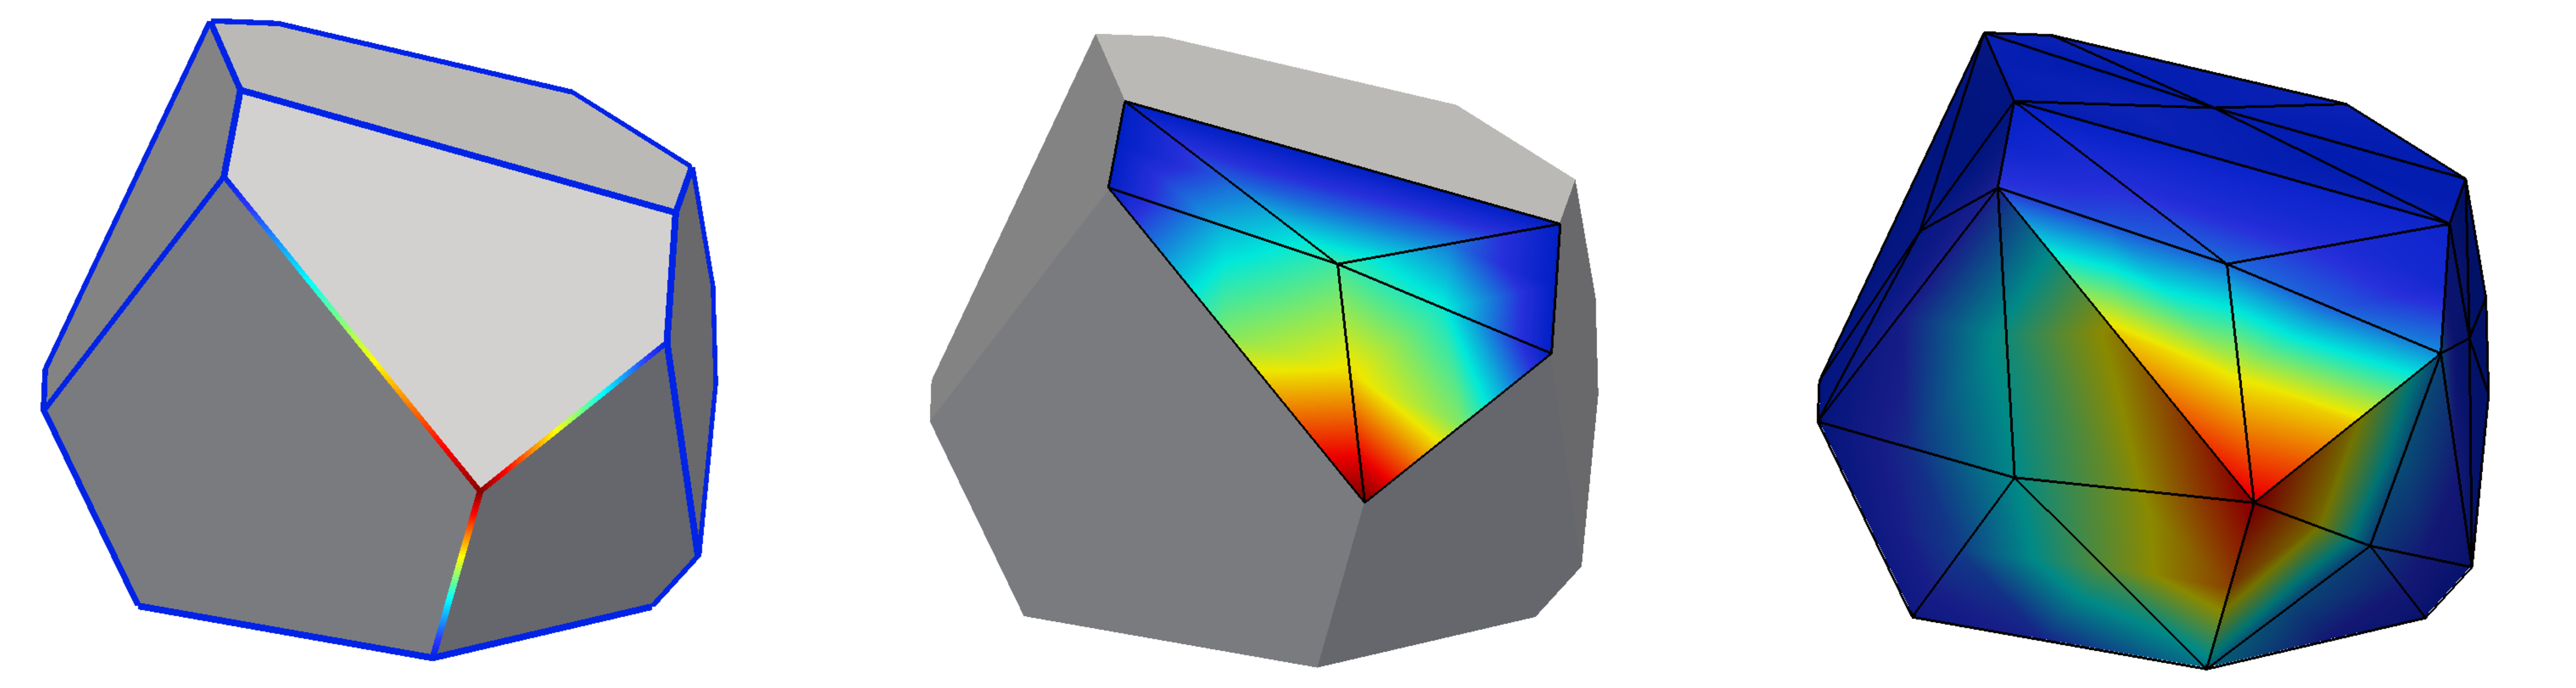
\includegraphics[width = 6.0in]{figures/harmonic_fem_sfs.pdf}
	\caption{The finite element approximation to a given harmonic shape function, defined hierarchially on each edge, face, and the element.}
	\label{fig:harmonic_fem_sfs}
\end{figure}
	
	This approach can become computationally expensive if the elements are subdivided into an excessively large number of tetrahedra, in the event that more accurate approximations to the shape functions are desired. However, initial numerical investigations have suggested that relatively coarse tetrahedral sub-divisions of the elements provide sufficiently accurate results; further subdivision (tetrahedral $h-$refinement) does little to improve the overall accuracy of the approach.
	
	A natural extension of the method proposed by Bishop to higher-order serendipity elements would be to consider $p-$refinement of an element's tetrahedral subdivision to recover higher-order polynomial completeness, i.e. to guarantee $\mathcal{U}^h (\Omega) \supset P^k (\Omega)$ for some desired polynomial order $k$. Unfortunately, the construction of shape functions on a given element would likely bear a much higher computational cost with increasing polynomial degree. The specification of stable and accurate numerical quadratures would present an additional challenge.
	
	Yet another generalization would be to consider subdividing the elements into arbitrary polyhedra, and solving (\ref{eq:weak_poisson}) by means of the virtual element method. This would allow for a more natural collocation of quadrature cells with the specified subdivision, akin to the partitioned element method proposed in \cite{Rashid:12}.
	
	However, a particular complication arises for harmonic shape functions and their corresponding $C^0 (\Omega)$ approximations on irregularly shaped elements: the solution to Laplace's equation may possess extremely sharp gradients if the geometry of the element contains reflex corners or nearly degenerate features (i.e. short edges). A consequence of this is poor conditioning of the element's local stiffness matrix, leading to excessively stiff modes of deformation (locking), and issues of numerical conditioning in the linear solution process. For this reason, it becomes of interest to consider non-conforming approximations $\varphi^h \in \mathcal{U}^h (\Omega) \not\subset \mathcal{U} (\Omega)$ which have the potential to overcome these issues.
	
\subsection*{Non-conforming Galerkin Approximations to \\ Generalized Harmonic Shape Functions}

	If the boundary conditions imposed upon a given shape function are relaxed to the extent that $\varphi^h \neq \bar{\varphi}$ on $\partial \Omega$, then clearly $\mathcal{U}^h (\Omega) \not\subset \mathcal{U} (\Omega)$, and one must resort to the use of non-conforming approximation methods. In such cases, the boundary conditions must be imposed in a weak sense, such that $\varphi^h$ still converges to $\varphi$ as the dimension of the non-conforming approximation space $\mathcal{U}^h (\Omega)$ is increased. A number of potential weak enforcement strategies are suggested in the following sections.
	
	\subsubsection*{Weak Enforcement of Boundary Conditions via a Lagrange Multiplier Method}
	
	One possible approach would be to consider a Lagrange multiplier method, to weakly enforce the boundary condition $\varphi = \bar{\varphi}$ on $\partial \Omega$ via
	\begin{equation}
		\min_{\varphi, \, \lambda} \mathcal{L}(\varphi,\lambda),
	\end{equation}
	\begin{equation}
	\mathcal{L}(\varphi,\lambda) \equiv \frac{1}{2} \int_{\Omega} \nabla \varphi \cdot \nabla \varphi \, dV - \int_{\Omega} f_{\Omega} \, \varphi \, dV + \int_{\partial \Omega} \left[ \varphi - \bar{\varphi} \right] \lambda \, dA,
\end{equation}
	involving the specification of a Lagrange multiplier field $\lambda \in \Lambda (\partial \Omega) = \left\{ \lambda \in L^2 (\partial \Omega) \right\}$, and it's corresponding approximation $\lambda^h \in \Lambda^h (\partial \Omega) \subset \Lambda (\partial \Omega)$. Differentiation of the Lagrangian yields two sets of equations in terms of the approximations $\varphi^h \in \mathcal{U}^h (\Omega)$ and $\lambda^h \in \Lambda^h (\partial \Omega)$:
	\begin{equation}
		\int_{\Omega} \nabla \varphi^h \cdot \nabla \eta^h \, dV - \int_\Omega f_\Omega \eta^h \, dV + \int_{\partial \Omega} \lambda^h \eta^h \, dA = 0 \quad \forall \eta^h \in \mathcal{U}^h (\Omega),
	\end{equation}
	\begin{equation}
		\int_{\partial \Omega} (\varphi^h - \bar{\varphi}) \, \mu^h \, dA = 0 \quad \forall \mu^h \in \Lambda^h (\partial \Omega).
	\end{equation}
	Suppose finite-dimensional bases are established for $\mathcal{U}^h (\Omega)$ and $\Lambda^h (\partial \Omega)$, i.e.
\begin{equation}
	\varphi^h (\mathbf{X}) = \sum_{a=1}^{N} \psi_a (\mathbf{X}) \varphi_a, \quad \lambda^h (\mathbf{X}) = \sum_{a=1}^{M} \chi_a (\mathbf{X}) \lambda_a,
\end{equation}
such that
\begin{equation}
	\sum_{a=1}^N \left[ \int_{\Omega} \nabla \psi_a \cdot \nabla \psi_b \, dV \right] \varphi_a + \sum_{c=1}^M \left[ \int_{\partial \Omega} \psi_b \, \chi_c \, dA \right] \lambda_c = \int_{\partial \Omega} f_\Omega \, \psi_b \, dA \quad \forall b,
\end{equation}
\begin{equation}
	\sum_{b=1}^N \left[ \int_{\partial \Omega} \chi_c \, \psi_b \, dA \right] \varphi_b = \int_{\partial \Omega} \bar{\varphi} \, \chi_c \, dA \quad \forall c.
\end{equation}
Given an appropriate selection for the indicated bases, the determination of the unknowns ($\varphi_a$ and $\lambda_a$) entails the solution of a saddle-point system of equations, written in matrix-vector format:
\begin{equation}
	\left[ \begin{array}{cc} \mathbf{A} & \mathbf{B} \\ \mathbf{B}^T & \mathbf{0} \end{array} \right] \left\{ \begin{array}{c} \boldsymbol{\varphi} \\ \boldsymbol{\lambda} \end{array} \right\} = \left\{ \begin{array}{c} \mathbf{f} \\ \bar{\boldsymbol{\varphi}} \end{array} \right\},
\end{equation}
where
\begin{equation}
	A_{ab} = \int_{\Omega} \nabla \psi_a \cdot \nabla \psi_b \, dV, \quad B_{bc} = \int_{\partial \Omega} \psi_b \, \chi_c \, dA,
\end{equation}
\begin{equation}
	f_{b} = \int_{\partial \Omega} f_\Omega \, \psi_b \, dA, \quad \bar{\varphi}_{c} = \int_{\partial \Omega} \bar{\varphi} \, \chi_c \, dA.
\end{equation}

	The main advantage of this approach is that virtually any space of functions may be selected for $\mathcal{U}^h (\Omega)$, such that the resulting approximations $\varphi^h \in \mathcal{U}^h (\Omega)$ deliberately do not contain sharp gradients.
	
	Arguably the simplest (and most efficient) choice is $\mathcal{U}^h (\Omega) = P^{k} (\Omega)$, resembling certain formulations of the VETFEM (\cite{Rashid:00}, \cite{Rashid:06}) where the basis functions for the Lagrange multiplier field $\chi_c (\mathbf{X}) = \delta (\mathbf{X} - \mathbf{X}_c) \, \, \forall c = 1, \ldots, N_v$ are Dirac delta functions associated with the individual nodes of the element. A potential shortcoming of this particular choice for $\chi_c$ is that the resulting shape functions may yield sharp gradients along short element edges.
	
	Various other choices for the Lagrange multiplier basis are possible which may yield less spurious solutions (for instance $\Lambda^h (\partial \Omega) = P^{k} (\partial \Omega)$), though these may lead to ill-posedness of the saddle-point problem. More sophisticated linear solution methodologies are required in these cases.

	\subsubsection*{Weak Enforcement of Boundary Conditions via Nitsche's Method}
	
	As a viable alternative to the Lagrange multiplier method presented in the previous section, one may instead consider using Nitsche's method (refer to \cite{Juntunen&Stenberg:09}) as a means of weakly enforcing the boundary conditions for a given shape function, i.e.
	\begin{eqnarray}
		\int_{\Omega} \nabla \varphi^h \cdot \nabla \eta^h \, dV - \int_{\partial \Omega} \left[ \frac{\partial \varphi^h}{\partial N} \eta^h + \varphi^h \frac{\partial \eta^h}{\partial N} \right] \, dA + \frac{1}{\gamma |\partial \Omega|^{\beta}} \int_{\partial \Omega} \varphi^h \eta^h \, dA \nonumber \\ = \int_\Omega f_\Omega \, \eta^h \, dV - \int_{\partial \Omega} \bar{\varphi} \frac{\partial \eta^h}{\partial N} \, dA + \frac{1}{\gamma |\partial \Omega|^{\beta}} \int_{\partial \Omega} \bar{\varphi} \eta^h \, dA \quad \forall \eta^h \in \mathcal{U}^h (\Omega),
	\end{eqnarray}
	where $\gamma > 0$ is a stabilization parameter, $| \partial \Omega |$ denotes the surface area of $\partial \Omega$, and $\beta = (d-1)^{-1}$ for $\Omega \subset \mathbb{R}^d$, $d \geq 2$.
	
	Provided the stabilization parameter $\gamma$ is specified appropriately, the Galerkin approximation $\varphi^h$ to Nitsche's method can be obtained as the solution to the symmetric, positive-definite system of equations $\mathbf{A} \boldsymbol{\varphi} = \mathbf{f}$, where
	\begin{equation}
		A_{ab} = \int_{\Omega} \nabla \psi_a \cdot \nabla \psi_b \, dV - \int_{\partial \Omega} \left[ \frac{\partial \psi_a}{\partial N} \psi_b + \psi_a \frac{\partial \psi_b}{\partial N} \right] \, dA + \frac{1}{\gamma |\partial \Omega|^{\beta}} \int_{\partial \Omega} \psi_a \, \psi_b \, dA,
	\end{equation}
	\begin{equation}
		f_{b} = \int_{\Omega} f_\Omega \, \psi_b \, dV - \int_{\partial \Omega} \bar{\varphi} \frac{\partial \psi_b}{\partial N} \, dA + \frac{1}{\gamma |\partial \Omega|^{\beta}} \int_{\partial \Omega} \bar{\varphi} \, \psi_b \, dA.
	\end{equation}
	
	As discussed in the previous section, a rather natural choice for the space of approximating functions is $\mathcal{U}^h (\Omega) = P^{k} (\Omega)$. The resulting method yields reasonably well-conditioned stiffness matricies for convex shapes, even when the elements possess degenerate edges. However, experimental evidence suggests that for non-convex shapes, the resulting shape function approximations may succumb to Runge's phenomenon. Figure (L) depicts the results for increasing $k$.
	
	These considerations have led to the conclusion that piecewise approximation methods may provide a preferred means for constructing more well-behaved approximations. The remainder of our discussion will focus upon such methods.
	
\section{Piecewise Polynomial Approximations to \\ Generalized Harmonic Shape Functions}

Partitioned element methods consider the approximation to a given element's shape functions via piecewise polynomials defined over a partition of the element's domain. In this regard, the approach proposed by Bishop in \cite{Bishop:14} is properly regarded as a partitioned element method.

The eponymous partitioned element method introduced in \cite{Rashid:12} solves (\ref{eq:approximate_bvp}) by empolying an approximation scheme which closely resembles a stabilized virtual element method. Herein we propose an alternative approach based upon the interior penalty discontinuous Galerkin finite element method.

\subsection*{The Element Partition}

\begin{figure} [!ht]
	\centering
	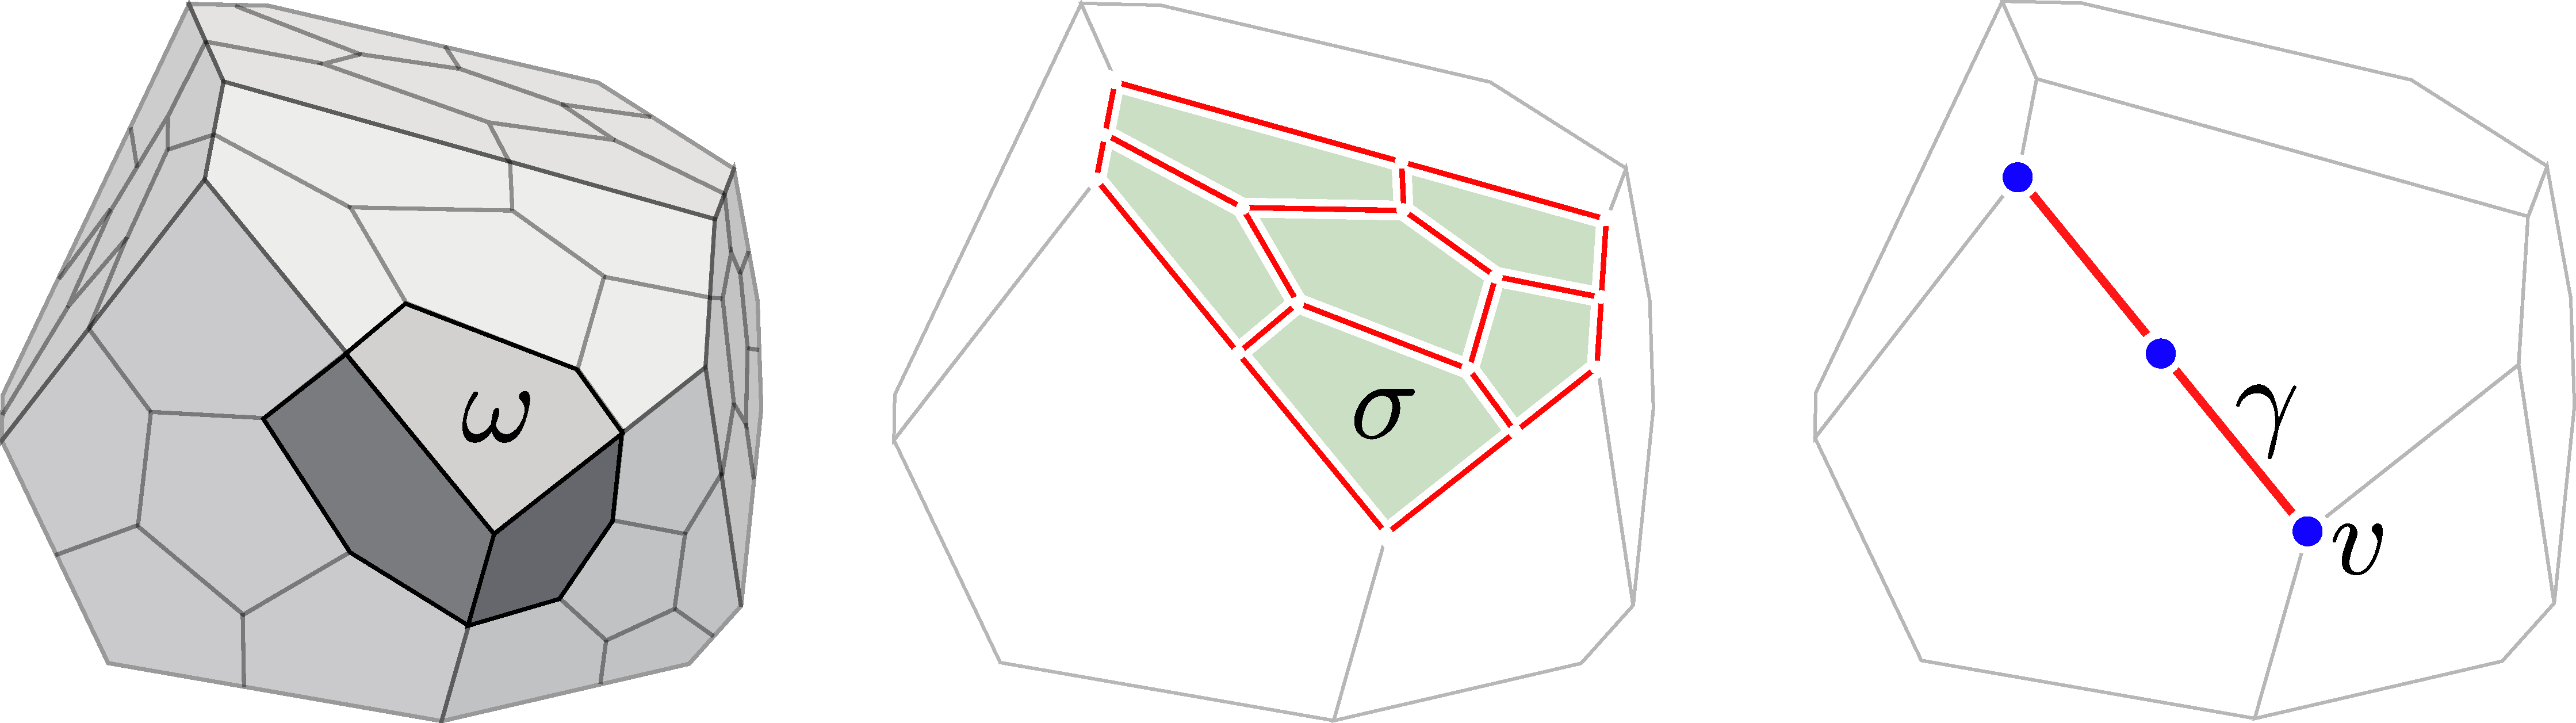
\includegraphics[width = 6.0in]{figures/polyhedron_partition.pdf}
	\caption{A representative polyhedral element $\Omega \subset \mathbb{R}^3$, and it's corresponding partition into cells, facets, segments, and verticies.}
	\label{fig:partitioned_element}
\end{figure}

	Consider a partition $\mathcal{T}_\omega (\Omega)$ of a given polyhedral element $\Omega$ into polyhedral cells $\omega \subset \Omega$. The boundary of each cell consists of polygonal facets $\sigma \subset \partial \omega$. Further, denote by $\Gamma_\omega$ the set of all interior cell interfaces (facets) shared by two adjacent cells, such that a given polygonal facet $\sigma$ belongs either to $\Gamma_\omega$ or the boundary of the element $\partial \Omega$.
	
	In turn, let $\mathcal{T}_{\sigma} (F)$ denote the partition of a given face $F \subset \partial \Omega$ into polygonal facets $\sigma \subset F$. The boundary of each facet consists of linear segments $\gamma \subset \partial \sigma$. For each face $F$, $\Gamma_\sigma$ shall denote the set of all interior facet interfaces (segments) shared by two facets belonging to $F$, such that a given linear segment $\gamma$ belongs either to $\Gamma_\sigma$ or $\partial F$.
	
	Finally, $\mathcal{T}_{\gamma} (E)$ denotes the partition of a given edge $E \subset \partial F$ into linear segments $\gamma \subset E$. The endpoints of each segment are called verticies $v \subset \partial \gamma$. For each edge $E$, $\Gamma_\gamma$ denotes the set of all interior segment interfaces (verticies) shared by two segments belonging to $E$, such that a given vertex $v$ belongs either to $\Gamma_\gamma$ or $\partial E$. Any vertex $v \in \partial E$ is also a node $v = V$.
	
	Several simple partitioning schemes are proposed:
	\begin{itemize}
		\item \textbf{Edge-based}: For star-convex shapes -- the vertex-averaged centroid is used to subdivide the element into triangles (in 2D) or tetrahedra (in 3D) which are associated with each linear edge of the element.
		\item \textbf{Node-based}: For arbitrary shapes -- the element is sub-divided into quadrature cells corresponding to the tributary area surrounding each node.
		\item \textbf{Voronoi}: For arbitrary shapes -- the element is sub-divided into Voronoi cells, whose corresponding voronoi sites are generated via a constrained maximal poisson-disk sampling process, as described in \cite{Ebeida:11}.
	\end{itemize}
	The aforementioned approaches are further illustrated in Figure \ref{fig:partitioning_types}.
	\begin{figure} [!ht]
		\centering
		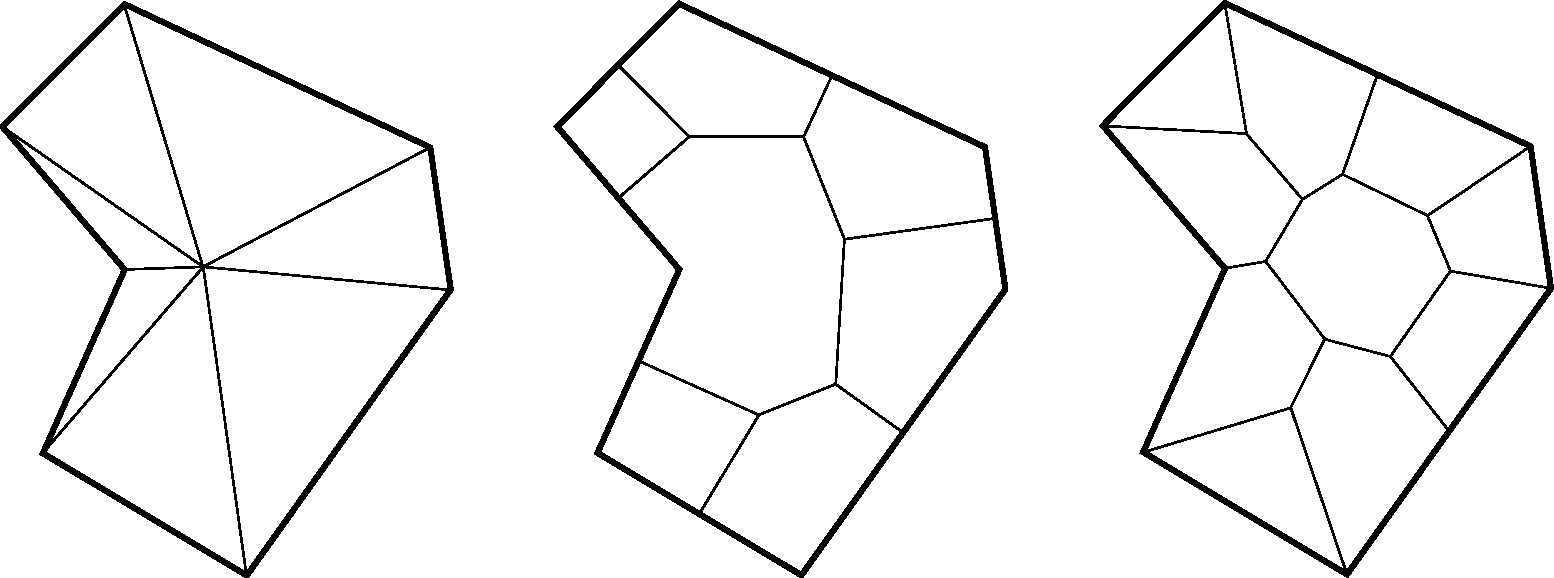
\includegraphics[width = 6.0in]{figures/partition_types.pdf}
		\caption{Polygonal element partitioning schemes, from left to right: edge-based partition, node-based partition, voronoi partition.}
		\label{fig:partitioning_types}
	\end{figure}
	
	We denote the volume of a given cell as $|\omega|$, the area of a facet as $|\sigma|$, and the length of a segment as $|\gamma|$. Each facet possesses an associated normal direction $\mathbf{N}_\sigma$, whose orientation is outward from $\Omega$ for all $\sigma \in \partial \Omega$. The orientation of $\mathbf{N}_\sigma$ is otherwise arbitrary for all $\sigma \in \Gamma_\omega$. Likewise, 

\subsection*{Discontinuous Galerkin Approximations to \\ Harmonic Shape Functions}

	Consider the broken Sobolev space $\mathcal{D}^h_k (\Omega) = \left\{ \varphi \in L^2 (\Omega) : \varphi|_{\omega} \in P^k (\omega) \, \forall \omega \in \mathcal{T}_\omega (\Omega) \right\}$ consisting of (discontinuous) piecewise polynomials defined over the partition of the element. The symmetric interior penalty discontinuous Galerkin method (SIPG) described in \cite{Riviere:08} is applied to (\ref{eq:weak_bvp}) to obtain approximations $\varphi^h \in \mathcal{D}^h_k (\Omega) \not\subset \mathcal{U} (\Omega)$ to generalized harmonic shape functions $\varphi \in \mathcal{U} (\Omega)$, satisfying
	\begin{eqnarray}
		\sum_{\omega \in \mathcal{T}_\omega (\Omega)} \int_{\omega} \nabla \varphi^h \cdot \nabla \eta^h \, dV - \sum_{\sigma \in \Gamma_\omega \cup \partial \Omega} \int_{\sigma} \bigg( \left\{ \frac{\partial \varphi^h}{\partial N_{\sigma}} \right\} [\![ \eta^h ]\!] + [\![ \varphi^h ]\!] \left\{ \frac{\partial \eta^h}{\partial N_{\sigma}} \right\}  \bigg) \, dA \nonumber \\ + J_0 (\varphi^h,\eta^h) + J_1 (\varphi^h,\eta^h) = \int_{\Omega} f_{\Omega} \, \eta^h \, dV + \sum_{\sigma \in \partial \Omega} \int_{\sigma} \left(\frac{\alpha_{\sigma0}}{|\sigma|^{\beta_0}} \eta^h - \frac{\partial \eta^h}{\partial N_{\sigma}} \right) \bar{\varphi} \, dA
		\label{eq:dg_poisson}
	\end{eqnarray}
	for all $\eta^h \in \mathcal{D}^h_k (\Omega)$, where
	\begin{equation}
		\{ \varphi \} = \frac{1}{2} (\varphi|_{\omega_1} + \varphi|_{\omega_2}), \quad [\![ \varphi ]\!] = (\varphi|_{\omega_1} - \varphi|_{\omega_2}) \quad \forall \sigma = \partial \omega_1 \cap \partial \omega_2,
	\end{equation}
	\begin{equation}
		\{ \varphi \} = [\![ \varphi ]\!] = \varphi|_{\omega} \quad \forall \sigma = \partial \omega \cap \partial \Omega,
	\end{equation}
	and where
	\begin{equation}
		J_0 (\varphi^h,\eta^h) = \sum_{\sigma \in \Gamma_\omega \cup \partial \Omega} \frac{\alpha_{\sigma0}}{|\sigma|^{\beta_0}} \int_{\sigma} [\![ \varphi^h ]\!] \, [\![ \eta^h ]\!] \, dA,
	\end{equation}
	\begin{equation}
		J_1 (\varphi^h,\eta^h) = \sum_{\sigma \in \Gamma_\omega} \frac{\alpha_{\sigma1}}{|\sigma|^{\beta_1}} \int_{\sigma} \left[\!\!\left[ \frac{\partial \varphi^h}{\partial N_{\sigma}} \right]\!\!\right] \, \left[\!\!\left[ \frac{\partial \eta^h}{\partial N_{\sigma}} \right]\!\!\right] \, dA.
	\end{equation}
	$J_0 (\varphi^h,\eta^h)$ and $J_1 (\varphi^h,\eta^h)$ are supplementary bilinear forms which penalize jumps in the indicated functions' values and their normal derivatives at cell boundaries. The parameters $\alpha_{\sigma0}$, $\beta_0$, must be appropriately specified such that $\alpha_{\sigma0} > 0$ is sufficiently large, and $\beta_0 (d-1) \geq 1$ where $\Omega \subset \mathbb{R}^d$, $d \geq 2$; the specification of $\alpha_{\sigma1}$, $\beta_1$ is less strict, allowing for $\alpha_{\sigma1} \geq 0 \, \, \forall \sigma$.
	
	If one considers a non-dimensional analysis where $\mathbf{X} = h_\Omega \mathbf{X}'$, and $h_\Omega$ denotes a characteristic length scale corresponding to the diameter of the element $\Omega$, the following quantities may be expressed in terms of their non-dimensional counterparts:
    \begin{equation}
        dV = h_\Omega^d dV', \quad dA = h_\Omega^{d-1} dA', \quad \nabla = h_\Omega^{-1} \nabla', \quad |\sigma| = h_\Omega^{d-1} |\sigma'|, \quad f_{\Omega} = h_\Omega^{-2} f_{\Omega'}.
    \end{equation}
    It is presumed that $\alpha_{\sigma0}$, $\alpha_{\sigma1}$ are defined independently of $h_\Omega$. Consequently,
    \begin{align}
		h_\Omega^{d-2} & \left[ \sum_{\omega' \in \mathcal{T}_{\omega'} (\Omega')} \int_{\omega'} \nabla' \varphi^h \cdot \nabla' \eta^h \, dV' - \int_{\Omega'} f_{\Omega'} \, \eta^h \, dV' + \sum_{\sigma' \in \partial \Omega'} \int_{\sigma'} \frac{\partial \eta^h}{\partial N_{\sigma'}} \, \bar{\varphi} \, dA' \right. \nonumber \\ 
		& \left. - \sum_{\sigma' \in \Gamma_{\omega'} \cup \partial \Omega'} \int_{\sigma'} \bigg( \left\{ \frac{\partial \varphi^h}{\partial N_{\sigma'}} \right\} [\![ \eta^h ]\!] + [\![ \varphi^h ]\!] \left\{ \frac{\partial \eta^h}{\partial N_{\sigma'}} \right\}  \bigg) \, dA' \right] \nonumber \\ 
		+ \, h_\Omega^{(d-1)(1-\beta_0)} & \left[ \sum_{\sigma' \in \Gamma_{\omega'} \cup \partial \Omega'} \frac{\alpha_{\sigma0}}{|\sigma'|^{\beta_0}} \int_{\sigma'} [\![ \varphi^h ]\!] \, [\![ \eta^h ]\!] \, dA' - \sum_{\sigma' \in \partial \Omega'} \frac{\alpha_{\sigma0}}{|\sigma'|^{\beta_0}} \int_{\sigma'} \eta^h \, \bar{\varphi} \, dA' \right] \nonumber \\ 
		+ \, h_\Omega^{(d-1)(1-\beta_1)-2} & \left[ \sum_{\sigma' \in \Gamma_{\omega'}} \frac{\alpha_{\sigma1}}{|\sigma'|^{\beta_1}} \int_{\sigma'} \left[\!\!\left[ \frac{\partial \varphi^h}{\partial N_{\sigma'}} \right]\!\!\right] \, \left[\!\!\left[ \frac{\partial \eta^h}{\partial N_{\sigma'}} \right]\!\!\right] \, dA' \right] = 0 \quad \forall \eta^h \in \mathcal{D}^h_k (\Omega). 
		\label{eq:dg_nondim}
	\end{align}
	To maintain dimensional consistency, it is suggested that $\beta_0$ and $\beta_1$ be chosen such that
	\begin{equation}
		\beta_0 = (d-1)^{-1}, \quad \beta_1 = -(d-1)^{-1}.
	\end{equation}
	
	To ensure that the resulting linear system of equations is reasonably well-conditioned, the penalty parameters $\alpha_{\sigma0}$, $\alpha_{\sigma1}$ should not be made excessively large. Nonetheless, an interesting limiting case occurs when $\alpha_{\sigma0}, \alpha_{\sigma1} \rightarrow \infty$ proportionally:
	\begin{eqnarray}
		J_0 (\varphi^h,\eta^h) + J_1 (\varphi^h,\eta^h) = \sum_{\sigma \in \partial \Omega} \frac{\alpha_{\sigma0}}{|\sigma|^{\beta_0}} \int_{\sigma} \eta^h \,  \bar{\varphi} \, dA \quad \forall \eta^h \in \mathcal{D}^h_k (\Omega).
		\label{eq:pure_penalty}
	\end{eqnarray}
	Under certain conditions (for particular choices of $\mathcal{T}_\omega (\Omega)$ and $\mathcal{D}^h_k (\Omega)$), the above weak form may in fact yield a unique solution $\varphi^h$. However, the bilinear form arising from the penalty terms $J_0$ and $J_1$ alone is not guaranteed to be elliptic, in general.
	
	The majority of our subsequent analyses will explore the family of 3-parameter methods arising from
	\begin{equation}
		\alpha_{\sigma 0} = \alpha_{0}|_{\partial \Omega} \, \, \forall \sigma \in \partial \Omega, \quad \alpha_{\sigma 0} = \alpha_{0}|_{\Gamma_{\omega}} \, \, \forall \sigma \in \Gamma_{\omega}, \quad \alpha_{\sigma 1} = \alpha_{1}|_{\Gamma_{\omega}} \, \, \forall \sigma \in \Gamma_{\omega},
	\end{equation}
	entailing a separate penalization of the boundary condition via $\alpha_{0}|_{\partial \Omega}$. Decreasing the value of $\alpha_{0}|_{\partial \Omega}$ is tantamount to relaxing the degree to which the boundary condition is enforced, the effect of which will be examined and discussed later on.
	
%	Ultimately, one must show either that $\mathcal{S}^h$ and $\mathcal{V}^h$ and sub-spaces of $\mathcal{S}$ and $\mathcal{V}$, or else that any exterior approximation methods converge to the exact solution under cell refinement. Moreover, we must show that any approximation to the exact solution will yield elements that exhibit convergence under mesh (element) refinement -- an interesting embedded convergence problem.
		
	% Present the BVP (Laplace's equation) for polytopes with BCs
	% Various methods have sought solutions to the above using FEM, etc.
	% Such methods can be considered partitioned element methods
	% In those contexts, SFs more honest if partition is very fine
	% In the present work, we wish to consider relatively coarse pratitions
	% Question: how much refinement is actually necessary for convergence?
	% Answer: ostensibly not much at all, but it is important for stability
	% Caveat: depends on the order of completeness of the local PEM space
		% Linearly complete PEM spaces needed for 1st order convergence
		% For higher order convergence, can use h- or p-refinement
			% p-refinement is generally more efficient
			
	% May solve Laplace's equation directly with exact satisfaction of BCs
	% Or may modify the BCs in a suitable way to relax exact conformity
	% Must do so in a way that preserves:
		% Stability: must maintain ellipticity of local bilinear form
		% Completeness: reproduce low-order polynomials exactly
		% Weak Compatibility: pass generalized patch test, or equivalent
	% May accomplish this via a BC filtering/projection scheme
		% Effectively equivalent to enforcing BCs with Lagrange multipliers
		% Must carefully choose the basis for the Lagrange multiplier field
			% Must yield stability, completeness, weak compatibility
		% One option is a low-order polynomial sub-space
			% Effectively equivalent to using a low-order polynomial basis
			% This is precisely the result obtained by the VETFEM
			% Runs the risk of Runge's phenomenon
			% Using polynomial basis can lead to poor conditioning
			% Requires inefficient specification of polynomial space
		% Some issues could be avoided with use of FE basis on interior
			% Still, must choose polynomial basis carefully
			% This will be truly difficult for arbitrary polytopes
		% Another option is to use Lagrange multiplier field = nodal basis
			% Produces a naturally stable enforcement of BCs
				% Get a bijection between image and preimage of BCs
			% Problem: it may still be too strong
				% Effectively may be enforcing original BCs
			% Could introduce stabilization to zero block of system
				% Introduces an auxiliary penalty parameter
				% Stabilizes the saddle point problem
				% Smooths out the multiplier field
				% Practically equivalent to damping higher polynomials
	% Alternatively, may use a penalty method
		% Use adjustable parameter to damp out higher-order polynomials
		% Preserve behavior of low-order polynomials for convergence
		% Easy to demonstrate stability for parameter values > 0
		% Problem is how to set this parameter
			% Ostensibly will be more sensitive for degenerate geometries

%\subsection*{The Element Partition}

	%consider an arbitrary element domain
	%discretize domain into conforming sub-domains: a partition
	%limitation: sub-domains must be polytopes
	%shape constraints imposed according to chosen approx. method

%\begin{itemize}
%	\item Provide a figure of an element with partitioned geometry
%	\item Define partitioned geometry terms (cells, facets, segments, verticies, etc.), perhaps even give a table of definitions, all referring back to the main figure(s)
%	\item 
%\end{itemize}

%\subsection{Partition-Based Approximation Spaces}

		%define SFs as FE-like piece-wise polynomials on the partition
		%try to minimize number of basis functions for efficiency
%		\subsubsection*{FE basis}
			%unknowns stored at verticies only (efficient)
			%easy generalization to high order
			%limited to canonical shapes (tris/tets, quads/hexas)
			%quadrature rules much simpler (may use high order)
			%equivalent to Joe Bishop's approach (w/ Laplace SFs)
			%less sensitive to conditioning problems
%		\subsubsection*{WG basis}
			%unknowns stored on cells and edges
			%generalization to high order more expensive
			%Rashid & Sadri 2012 approach (low order)
			%may suffer from conditioning issues at high order
%		\subsubsection*{DG basis}
			%unknowns stored on cells
			%easy generalization to high order
			%New/current approach
			%may suffer from conditioning issues at high order
%		\subsubsection*{VE basis}
			%unknowns stored at verticies only (efficient)
			%high order generalization effected via serendipity SFs
			%generalizes to arbitrary polytopes
			%New/speculated approach
			%less sensitive to conditioning problems

%Traditional approximation methods typically consider the independent specification of two principal transformations: an interpolation scheme, which is necessary to represent field variables according to known point-values; and a quadrature rule, for the purposes of integrating such fields over the domain on which they are defined.

%In mathematical terms, an interpolant $\varphi$ is a linear operator which maps vectors $\mathbf{u} \in \mathbb{R}^k$ containing point-wise data regarding a field into scalar functions $f \in V^k (\Omega)$, i.e.
%\begin{equation}
%  \varphi \colon \mathbb{R}^k \mapsto V^k (\Omega)
%\end{equation}
%where $\mathbb{R}^k$ is a $k$-dimensional real space, and $V^k (\Omega)$ is a $k$-dimensional function space defined on $\Omega$.

%By constrast, a quadrature rule $\Sigma$ is a linear operator which maps scalar functions $f \in V^k (\Omega)$ to vectors $\mathbf{q} \in \mathbb{R}^p$ identifying point-wise samples of $f$, i.e.
%\begin{equation}
%  \Sigma \colon V^k (\Omega) \mapsto \mathbb{R}^p
%\end{equation}

%The composition $\Sigma \circ \varphi$ of an interpolant $\varphi$ with a quadrature rule $\Sigma$ yields a linear operator
%\begin{equation}
%  \Sigma \circ \varphi \colon \mathbb{R}^k \mapsto \mathbb{R}^p
%\end{equation}

\section{Partition-Based Quadrature Rules}

		%quadrature rules are defined/linked to the chosen partition
		%1-to-1 relation between partitioned cells and quadrature points
		%use Lassere integration to get weights of polytopal domains
		%employ low-order quadrature rules for the sake of efficiency
		%FE/simplicial discretization allows high-order composite rules
		
% need to integrate weak form terms on polytopes and their boundaries
	% must account for nonlinear kinematic and material behavior
	% must guarantee sufficient stability (inf-sup)
	% must be sufficiently accurate (Galerkin exactness)
If arbitrary polytopal shapes are to be used as elements in the PEM, then there arises a need for devising a means of integrating contributions to the weak form, ostensibly through the use of domain quadrature rules. Such rules must be sufficiently stable (utilizing a sufficient number of well-positioned quadrature points) and accurate (capable of exactly integrating low-order polynomials up to some specified degree).
	
% PEM approaches this task with the aid of partition-based quadrature rules
	% Elements are partitioned/discretized into sub-domains
		% Number of sub-domains should be sufficient to guarantee stability
	% Quadrature rules are defined on each sub-domain
	% Composite quadrature rules are assembled by considering these quadratures taken together
Partitioned element methods approach this task by partitioning the elements (and their boundaries) into a sufficient number of polytopal sub-domains which are used as integration cells. Low-order (i.e. 1-point) quadrature rules are defined on each of these sub-domains, and a composite quadrature rule for the element is constructed from the resulting sets of quadrature points. In general, these rules will need to be modified to satisfy Galerkin exactness for certain low-order polynomial solutions.
	
% Quadrature rules are adjusted after-the-fact by considering an exact integration of low-order polynomial terms to guarantee Galerkin exactness
	% may be viewed as a type of gradient correction measure
	% applied to each quadrature (interior and boundary) separately
% discuss particular in the following sub-sections:
Methods for partitioning the elements into sub-domains which yield stable and efficient composite quadrature rules are discussed in the following section. A discussion is given later on to the correction of these quadratures for the sake of satisfying Galerkin exactness (quadrature consistency).
		
	\subsection*{Composite Quadrature Rules}
	
	Given a partition of an element into polytopal sub-domains (quadrature cells), one may utilize low order quadrature rules over each sub-domain, thereby yielding a composite quadrature rule over the element as a whole, whose overall accuracy is determined by the order of accuracy used in each sub-domain.
	
	The simplest quadrature rule of this form is the composite mid-point scheme, where the quadrature points are located at the centroids of each sub-domain. Such a rule exactly integrates polynomials up to first order, and is reasonably accurate, otherwise. The integration points are guaranteed to be interior to each sub-domain (and the element as a whole), provided each cell is convex.
	
	For simple sub-divisions (consisting of triangles or tetrahedra), composite quadrature rules may be extended rather naturally to obtain higher-order accuracy. For generic sub-divisions (consiting of arbitrary polytopes), the extension to high-order is not as straight-forward. For this reason, subsequent discussions will be concerned almost exclusively with composite mid-point rules.
	
	The weights and locations of a composite mid-point quadrature rule correspond to the volumes and geometric centroids of each cell. In general, a given quadrature cell $\omega$ may be an arbitrary polyhedron, whose volume $|\omega|$ and centroid $\bar{\mathbf{X}}$ may be computed using the $0$-th and $1$-st order moments of $\omega$, i.e.
	\begin{equation}
		|\omega| = \int_{\omega} dV, \quad \bar{\mathbf{X}} = \frac{\int_{\omega} \mathbf{X} \, dV}{\int_{\omega} dV}.
	\end{equation}
	Using the method proposed by Chin et al. in \cite{Chin:15}, the computation of monomial moments of arbitrary degree $|\alpha|$ may be effected via an integral over $\partial \omega$:
	\begin{equation}
		\int_{\omega} \mathbf{X}^\alpha \, dV = \frac{1}{d+|\alpha|} \int_{\partial \omega} (\mathbf{X} \cdot \mathbf{N}) \, \mathbf{X}^\alpha \, dA,
	\end{equation}
	for any arbitrary polytope $\omega \subset \mathbb{R}^d$. If $\partial \omega$ may be partitioned into a collection of $d-1$ dimensional facets $\sigma \subset \partial \omega$, then
	\begin{equation}
		\int_{\omega} \mathbf{X}^\alpha \, dV = \frac{1}{d+|\alpha|} \sum_{\sigma \in \partial \omega} \int_{\sigma} (\mathbf{X} \cdot \mathbf{N}_{\sigma}) \, \mathbf{X}^\alpha \, dA,
	\end{equation}
	where $\mathbf{N}_\sigma$ is the outward (with respect to $\omega$) unit normal associated with facet $\sigma$. We remark that any location $\mathbf{X}$ positioned on a given facet $\sigma$ may be expressed as
	\begin{equation}
		\mathbf{X} = \mathbf{X}_\sigma + \sum_{i=1}^{d-1} X_i \, \hat{\mathbf{X}}_i,
	\end{equation}
	where $\mathbf{X}_\sigma$ is any reference location positioned on the hyperplane which contains $\sigma$, and $\hat{\mathbf{X}}_i$ form a parameterization of the in-plane coordinates on $\sigma$. This leads to the observation $\mathbf{X} \cdot \mathbf{N}_\sigma = \mathbf{X}_\sigma \cdot \mathbf{N}_\sigma \, \, \forall \mathbf{X} \in \sigma$, and thus
	\begin{equation}
		\int_{\omega} \mathbf{X}^\alpha \, dV = \frac{1}{d+|\alpha|} \sum_{\sigma \in \partial \omega} (\mathbf{X}_\sigma \cdot \mathbf{N}_{\sigma}) \int_{\sigma} \, \mathbf{X}^\alpha \, dA.
	\end{equation}
	The integral of $\mathbf{X}^\alpha$ over each facet may in turn be carried out via
	\begin{equation}
		\int_{\sigma} \mathbf{X}^\alpha \, dA = \frac{1}{d-1+|\alpha|} \left[ \sum_{\gamma \in \partial \sigma} \big( (\mathbf{X}_\gamma-\mathbf{X}_\sigma) \cdot \mathbf{N}_{\gamma} \big) \int_{\gamma} \mathbf{X}^\alpha \, dS + \mathbf{X}_\sigma \cdot \int_{\sigma} \nabla \mathbf{X}^\alpha \, dA \right],
	\end{equation}
	and the integral over each segment is
	\begin{equation}
		\int_{\gamma} \mathbf{X}^\alpha \, dS = \frac{1}{d-2+|\alpha|} \left[ \sum_{v \in \partial \gamma} \big( (\mathbf{X}_v-\mathbf{X}_\gamma) \cdot \mathbf{N}_{v} \big) \mathbf{X}^\alpha_v + \mathbf{X}_\gamma \cdot \int_{\gamma} \nabla \mathbf{X}^\alpha \, dS \right].
	\end{equation}
	
	Similarly defined composite rules may be defined on each polygonal face of a given polyhedral element, or on each edge of a polygonal element. However, while composite mid-point quadrature rules are able to provide reasonable accuracy, they will not necessarily lead to quadrature consistency, as expressed in (\ref{eq:quadrature_consistency}). For this reason, a gradient correction scheme (such as the one proposed by Bishop in \cite{Bishop:14}, or by Talischi in \cite{Talischi:15}) must be employed. Alternatively, a novel approach to restore quadrature consistency is presented in the following section.
		
	\subsection*{Selective Modal Quadrature}
	
	Consider all functions $f \in L^2 (\Omega)$ represented over an arbitrary polytopal element domain $\Omega \subset \mathbb{R}^d$. Standard quadrature rules approximate the integral of $f$ over $\Omega$ as
	\begin{equation}
		\int_\Omega f \, dV \approx \sum_{q=1}^{N_{qp}} w_q f(\mathbf{x}_q).
	\end{equation}
	Borrowing from notation typical of the VEM, consider an $L^2 (\Omega)$ polynomial projection operator $\Pi^{\Omega}_k : L^2 (\Omega) \mapsto P^k (\Omega)$ which may be used to decompose $f = f_p + f_n$ into polynomial and non-polynomial parts:
	\begin{equation}
		f_p = \Pi^{\Omega}_k f, \quad f_n = f - \Pi^{\Omega}_k f = \pi^{\Omega}_k f,
	\end{equation}
	where $\pi^{\Omega}_k : L^2 (\Omega) \mapsto L^2 (\Omega) \backslash P^k (\Omega)$. Consequently, we observe that $\Pi^{\Omega}_k f$ is $L^2 (\Omega)$ orthogonal to any $\pi^{\Omega}_k g$ for all $g \in L^2 (\Omega)$, to the extent that
	\begin{equation}
		\int_{\Omega} (\Pi^{\Omega}_k f) (g - \Pi^{\Omega}_k g) \, dv = \langle \Pi^{\Omega}_k f, g - \Pi^{\Omega}_k g \rangle_{\Omega} = 0 \quad \forall f, \, g \in L^2 (\Omega).
	\end{equation}
	
	We propose a quadrature rule of the form:
	\begin{equation}
		\int_\Omega f \, dV \approx \int_\Omega f_p \, dV + \sum_{q=1}^{N_{qp}} w_q f_n(\mathbf{x}_q),
	\end{equation}
	where it is supposed that the projection operators $\Pi^{\Omega}_k$ and $\pi^{\Omega}_k$ are well-defined on $\Omega$, and $\int_\Omega f_p \, dV$ may be computed exactly using the methodology proposed by Chin et al. in \cite{Chin:15}. Furthermore, if we wish to integrate the product $f g$ where $f, \, g \in L^2 (\Omega)$, we may write
	\begin{equation}
		\int_\Omega f g \, dV = \langle f, g \rangle_{\Omega} = \langle \Pi^{\Omega}_k f + \pi^{\Omega}_k f, \Pi^{\Omega}_k g + \pi^{\Omega}_k  g \rangle_{\Omega},
	\end{equation}
	which, by the linearity of the $L^2 (\Omega)$ inner product, and by the orthogonality of $\Pi^{\Omega}_k f$ and $\pi^{\Omega}_k g$ (and of $\pi^{\Omega}_k f$ and $\Pi^{\Omega}_k g$), yields
	\begin{equation}
		\int_\Omega f g \, dV = \langle \Pi^{\Omega}_k f, \Pi^{\Omega}_k g \rangle_{\Omega} + \langle \pi^{\Omega}_k f, \pi^{\Omega}_k g \rangle_{\Omega},
	\end{equation}
	and thus
	\begin{equation}
		\int_\Omega f g \, dV \approx \int_\Omega f_p g_p \, dV + \sum_{q=1}^{N_{qp}} w_q f_n(\mathbf{x}_q) g_n(\mathbf{x}_q).
	\end{equation}
	This is effectively equivalent to integrating the product of all low-order polynomials exactly, while integrating the product of all non-polynomial ``remainders'' approximately, using a quadrature rule.
	
	If we are only given evaluations of a function $f$ at a set of discrete (quadrature) points $\left\{ \mathbf{x}_q \right\}_{q=1}^{N_{qp}}$, then we must construct a low-order polynomial projection operator by considering the least-squares problem:
	\begin{equation}
		\min_{f_p \in P^k (\Omega)} \frac{1}{2} || f_p - f ||^2_\Omega,
	\end{equation}
	where $|| f ||_\Omega = \sqrt{\langle f, f \rangle_\Omega}$ is deliberately approximated using the element's quadrature rule:
	\begin{equation}
		\langle f, f \rangle_\Omega \approx \sum_{q=1}^{N_{qp}} w_q \left[ f(\mathbf{x}_q) \right]^2.
		\label{eq:L2projection}
	\end{equation}
	For a given polynomial basis $\left\{ z_a \right\}_{a=1}^{K}$ which spans $P^k (\Omega)$, we may write
	\begin{equation}
		f_p (\mathbf{x}) = \sum_{a=1}^{K} z_a (\mathbf{x}) c_a = \mathbf{z}^T (\mathbf{x}) \, \mathbf{c},
	\end{equation}
	and the solution to (\ref{eq:L2projection}) satisfies
	\begin{equation}
		\sum_{a=1}^{K} \sum_{q=1}^{N_{qp}} w_q z_b (\mathbf{x}_q) z_a (\mathbf{x}_q) c_a =
		\sum_{q=1}^{N_{qp}} w_q z_b (\mathbf{x}_q) f(\mathbf{x}_q) \quad \forall b = 1, \, \ldots, \, K,
	\end{equation}
	The above may be written in matrix-vector format as $\mathbf{Z}^T \mathbf{W} \mathbf{Z} \mathbf{c} = \mathbf{Z}^T \mathbf{W} \mathbf{f}$, where we denote $f_i = f(\mathbf{x}_i)$, $W_{ii} = w_i, \, W_{ij} = 0 \, \forall i \neq j$, and $Z_{ij} = z_j (\mathbf{x}_i)$. The discrete polynomial projection operator $\mathbf{\Pi}^{\Omega}_k : \mathbb{R}^{N_{qp}} \mapsto \mathbb{R}^K$ is computed as $\boldsymbol{\Pi}^{\Omega}_k = (\mathbf{Z}^T \mathbf{W} \mathbf{Z})^{-1} \mathbf{Z}^T \mathbf{W}$, and the complement operator $\boldsymbol{\pi}^{\Omega}_k : \mathbb{R}^{N_{qp}} \mapsto \mathbb{R}^{N_{qp}}$ is $\boldsymbol{\pi}^{\Omega}_k = \mathbf{1}_{N_{qp}} - \mathbf{Z} \boldsymbol{\Pi}^{\Omega}_k$. Consequently,
	\begin{equation}
		\langle \Pi^{\Omega}_k f, \Pi^{\Omega}_k g \rangle_{\Omega} = \langle \mathbf{z}^T \boldsymbol{\Pi}^{\Omega}_k \mathbf{f}, \mathbf{z}^T \boldsymbol{\Pi}^{\Omega}_k \mathbf{g} \rangle_{\Omega} = \mathbf{f}^T \left[ {\boldsymbol{\Pi}^{\Omega}_k}^T \left( \int_{\Omega} \mathbf{z} \otimes \mathbf{z} \, dV \right) \boldsymbol{\Pi}^{\Omega}_k \right] \mathbf{g},
	\end{equation}
	\begin{equation}
		\langle \pi^{\Omega}_k f, \pi^{\Omega}_k g \rangle_{\Omega} \approx \sum_{q=1}^{N_{qp}} w_q f_n(\mathbf{x}_q) g_n(\mathbf{x}_q) = \mathbf{f}^T \left[ {\boldsymbol{\pi}^{\Omega}_k}^T \mathbf{W} \boldsymbol{\pi}^{\Omega}_k \right] \mathbf{g},
	\end{equation}
	and thus
	\begin{equation}
		\int_\Omega f g \, dV \approx \mathbf{f}^T \mathbf{M}_k \mathbf{g} = \sum_{q = 1}^{N_{qp}} \sum_{p = 1}^{N_{qp}} M_k (\mathbf{x}_q,\mathbf{x}_p) \, f (\mathbf{x}_q) \, g (\mathbf{x}_p),
	\end{equation}
	\begin{equation}
		\mathbf{M}_k \equiv \left[ {\boldsymbol{\Pi}^{\Omega}_k}^T \left( \int_{\Omega} \mathbf{z} \otimes \mathbf{z} \, dV \right) \boldsymbol{\Pi}^{\Omega}_k \right] + \left[ {\boldsymbol{\pi}^{\Omega}_k}^T \mathbf{W} \boldsymbol{\pi}^{\Omega}_k \right].
	\end{equation}
	
	We shall refer to this form of integration as \textit{selective modal quadrature}, given that the products of particular low-order polynomial modes are integrated exactly, and the products of any higher-order modes are approximated using the element's quadrature rules. The advantage of modal quadrature is that we may exactly integrate any terms which directly impact quadrature consistency. Consequently, nearly any stable numerical integration scheme (e.g. composite mid-point quadrature) may be used to integrate the higher-order products.
	
	Rather than storing the independent quadrature weights $w_q = w (\mathbf{x}_q)$, selective modal quadrature requires the storage of a generalized quadrature weighting matrix $M_k (\mathbf{x}_q,\mathbf{x}_p)$. Alternatively, for the sake of efficiency, if the function $g$ is known a priori (e.g. if $g$ is a test function for a weighted residual method), then we need only store the ``augmented'' test function values:
	\begin{equation}
		\tilde{g}^{(k)} (\mathbf{x}_q) = \sum_{p = 1}^{N_{qp}} \frac{M_k (\mathbf{x}_q,\mathbf{x}_p)}{w_q} \, g (\mathbf{x}_p),
	\end{equation}		
	and all integrals involving $f$ and $g$ may be carried out via
	\begin{equation}
		\int_\Omega f g \, dV \approx \sum_{q = 1}^{N_{qp}} \, w_q \, \tilde{g}^{(k)} (\mathbf{x}_q) \, f (\mathbf{x}_q).
	\end{equation}
	
	If applied to the stress divergence integral appearing in (\ref{eq:residual}), the resulting expression would resemble a gradient correction scheme in some respects, although it should be noted that the above procedure would need to be applied separately to each term appearing in the weak form (including boundary integrals). Specifically, the corresponding integration of the residual equations in (\ref{eq:residual}) would be carried out via
	\begin{equation}
		\int_{\mathcal{B}_0} P_{ij} \phi_{a,j} \, dV \approx \sum_{q=1}^{N_{qp}} w_q P_{ij} (\mathbf{x}_q) \tilde{\phi}^{(k)}_{a,j} (\mathbf{x}_q),
	\end{equation}
	\begin{equation}
		\int_{\mathcal{B}_0} \rho_0 b_i \phi_a \, dV \approx \sum_{q=1}^{N_{qp}} w_q \rho_0 (\mathbf{x}_q) b_i (\mathbf{x}_q) \tilde{\phi}^{(k-1)}_a (\mathbf{x}_q),
	\end{equation}
	\begin{equation}
		\int_{\Gamma^N_0} \bar{p}_i \phi_a \, dA \approx \sum_{b=1}^{N_{bp}} w_b  \bar{p}_i (\mathbf{x}_b) \tilde{\phi}^{(k)}_a (\mathbf{x}_b),
	\end{equation}
	where $\tilde{\phi}^{(k)}_a$ and $\tilde{\phi}^{(k)}_{a,j}$ denote the ``augmented'' test functions are their corresponding gradients, and $k$ is the indicated order of quadrature consistency (required to pass patch tests up to order $k+1$).

%\subsection{Selection of an Appropriate Objective Functional}

	%PEM BOUNDARY VALUE PROBLEMS
		%setup: define a space of approximating functions over the element (basis)
		%goal:  select shape functions from this basis that are "optimal"
			%trial functions should reproduce polynomials as best they can
			%test functions should be close to trial functions (for stability)
			%test functions should satisfy compatibility requirements weakly
			%test functions should satisfy quad. consistency requirements against polys.
		%must propose a positive-definite functional to minimize on E
		%must enforce constraints on minimization
			%consistency enforced via Lagrange multipliers
		%develop a resulting system of equations
		%condense out all internal dofs in terms of element nodal values
		%allows for the inclusion of optional enhanced dofs, if needed
		%want SFs to be free of pathologies
		%Laplace shape functions
			%Joe Bishop's approach
			%Rashid & Sadri 2012 approach
		%Least-squares penalty method
			%necessary to stabilize WG/DG approaches
		%Other methods
			%many things to explore in this regard...
			%biharmonic? (for higher-order completeness? C^1 hard)

%Once we have specified a given approximation space of functions, our goal is then to select the function from this space which best represents the nodal data that we are attempting to interpolate over the element. The essential question is this: by what metric should we objectively assess the appropriateness of a given approximating function?

%\subsection*{Construction of Element Appoximants}

%\section{Essential Requirements of the PEM}

%\subsection*{Reproducibility}

%Fundamentally, the approximation power of the PEM depends directly upon the degree of completeness of the underlying approximation space. In particular, the finite-dimensional trial solution space $\mathcal{S}^h$ should contain as a subspace $\mathbb{P}_k \subset \mathcal{S}^h$ for some $k \geq 0$, where $\mathbb{P}_k$ denotes the subspace of polynomial functions with maximal degree $k$. This guarantees that the PEM approximation space will be capable of exactly reproducing any polynomial function up to some specified order.

	%driven by completeness requirements
	%handled by BVP/functional specification
	%alternatively enforced via constraints

%\subsubsection*{Requirements of the Approximation Space}
%\subsection*{Compatibility}

	%driven by the generalized patch test
	%handled by constraints on approximation spaces/BVP



%\subsubsection*{Weak Compatibility}
%\subsection*{Stability}

		%driven by the inf-sup conditions
		%handled via sufficient quadrature arrangement

%\subsubsection*{Restrictions on the Element Partition}
%\subsection*{Variational Consistency}
%\subsubsection*{Weak Enforcement of Consistency}

		%driven by Galerkin exactness
		%enforced by quadrature accuracy
		%alternatively via lagrange multiplier constraint

%Recall the $\alpha$-th order variational consistency requirements:
%\begin{equation}
%  \int_\Omega \mathbf{x}^{\alpha} \varphi_{a,i} \, dv + \int_\Omega \mathbf{x}^{\alpha}_{,i} \varphi_a \, dv = \int_{\partial \Omega} \mathbf{x}^{\alpha} n_i \varphi_a \, da \quad \forall i, a.
%\end{equation}
%This degree of consistency is required for all $| \alpha | \leq k-1$ if the bi-linear form $a : \mathcal{S} \times \mathcal{V} \mapsto \mathbb{R}$ is to determine uniqueness of any exact polynomial solutions up to order $k$ contained within $\mathcal{S}^h \supset P_k$. Moreover, the above expression implies that any solution may be reasonably well approximated by low-order polynomials in the locality of the selected domain $\Omega$.

%Consequently, we may consider an application of the above consistency requirements to the entire problem domain $\Omega$, or -- more practically -- we may enforce consistency up to the desired order on each element domain $\Omega_e$. The element-local $\alpha$-th order consistency equations follow:
%\begin{equation}
%  \int_{\Omega_e} \mathbf{x}^{\alpha} \varphi_{a,i} \, dv + \int_{\Omega_e} \mathbf{x}^{\alpha}_{,i} \varphi_a \, dv = \int_{\partial \Omega_e} \mathbf{x}^{\alpha} n_i \varphi_a \, da \quad \forall i, a.
%  \label{eq:consistency3}
%\end{equation}

%In most practical situations, it may not be possible to evaluate the integral expressions exactly. Instead, numerical quadrature rules must be defined, both on the element's interior, and on its boundary, such that
%\begin{equation}
%  \int_{\Omega_e} f(\mathbf{x}) dv \approx \sum_{q=1}^{N_q} w_q f(\mathbf{x}_q), \quad \int_{\partial \Omega_e} f(\mathbf{x}) da \approx \sum_{b=1}^{N_b} w_b f(\mathbf{x}_b).
%\end{equation}
%This yields yet another form of consistency, henceforth referred to as ``quadrature consistency,'' expressed as:
%\begin{equation}
%  \sum_{q=1}^{N_q} w_q \left[ \mathbf{x}_q^{\alpha} \varphi^{(q)}_{a,i} + \mathbf{x}^{\alpha}_{q,i} \varphi^{(q)}_a \right] = \sum_{b=1}^{N_b} w_b \mathbf{x}_b^{\alpha} n^{(b)}_i \varphi^{(b)}_a \quad \forall i, a.
%  \label{eq:quadrature_consistency3}
%\end{equation}
%Moving forward in our developments, quadrature consistency will be the only form of consistency of practical interest, as it appropriately reflects the discrete data quantities at our disposal.

%A brief remark should be made regarding the lack of equivalence between the exact evaluation of consistency in equation (\ref{eq:consistency3}) and its numerical approximation in equation (\ref{eq:quadrature_consistency3}). In general, we cannot claim that satisfaction of one guarantees the other. There is only one occasion when we may say that (\ref{eq:quadrature_consistency3}) holds if and only if (\ref{eq:consistency3}) is satisfied, which occurs only when sufficiently accurate quadrature rules are used on the element and its boundary. In the vast majority of situations, however, this is an impractical constraint, as the construction of high-order quadrature rules on arbitrary polyhedra (though possible) proves to be somewhat computationally intensive (see the literature by Sukumar, etc.). Moreover, without a precise representation of the test functions over the element domain, it becomes infeasible to consider an exact integration of such functions.

%\subsection*{Numerical Quadrature Consistency}

%Beyond consistency with the weak form for a specified subspace of polynomial functions used to represent the solution, we also require that the numerical quadrature scheme utilized be sufficiently accurate to the extent that: Galerkin exactness is satisfied for certain classes of solutions, and that the quadrature error has a bound which is of a lower order than that of the approximation error.

%\subsubsection*{Bubnov-Galerkin and Petrov-Galerkin Approaches}

%\section{Specific Formulations}

%\subsection*{The Continuous-Galerkin PEM}

	% Harmonic SFs with an FE basis (Joe Bishop's approach)

%\subsection*{The Weak-Galerkin PEM}

	% Stabilized harmonic SFs with WG basis (Rashid & Sadri approach)

%\subsection*{The Discontinuous-Galerkin PEM}

	% C^k penalty approximating SFs with DG basis (new method)
	
%\subsection*{PEM Based on Composite Virtual Elements}

	% Harmonic SFs with VE basis + stabilization (new method)

%\section{Enhancements to Improve Solution Accuracy}

		%GENERAL RULE: enhancements should seek to increase completeness
			%witnessed in most incompatible modes formulations
			%only way to improve accuracy: increase order, locally
		%balance stability, consistency, compatibility, reproducibility
			%bubble function construction closely tied to other SFs
			%enhancements must be orthogonal to low-order terms
			%must satisfy compatibility weakly over whole boundary
		%element-wide high order enhancement functions
			%inexpensive way to improve polynomial completeness
			%may apply to boundary dofs, or internal dofs

%\subsection*{Partition-Based Enhancement Functions}
%\subsection*{Mixed PEM Discretizations}
